\section{Experimental Evaluation}
\label{sec:eval}
The evaluation checks whether the adaptation achieves strict DLA placement, what accuracy is retained, and how precision affects engine-plus-transfer latency, application-pipeline latency, and host-side cost. Module energy is measured separately at a matched 10\,Hz delivered rate. Each precision mode
includes stock YOLO11-n on GPU and with DLA+GPU fallback (stock fallback), and \model\ on GPU
and strict DLA. In the tables, DLA denotes strict placement for the adapted model.
Because \model\ on GPU and \model\ on strict DLA share the same weights, host
decoder, and NMS implementation, their difference isolates placement;
comparisons involving stock YOLO11-n also include architecture, training, and
prediction-interface differences.

\subsection{Platform and Precision Protocol}
\label{sec:setup}
Tests use an NVIDIA Jetson AGX Orin Developer Kit with L4T 36.4.4, CUDA 12.6,
and TensorRT 10.3 in NVIDIA's 50\,W mode with \texttt{jetson\_clocks} disabled.
All configurations use batch one and $640\times640$ inputs. FP16 enables
half precision; INT8 enables mixed INT8/FP16. These are build modes rather
than uniform operation precisions; GPU regions may retain FP16/FP32 intermediates.

Post-training calibration uses 500 COCO val2017 images sampled without
replacement with seed 2027, leaving 4,500 disjoint images for accuracy
\cite{lin2014coco}. Stock and adapted models are calibrated separately with
TensorRT's EntropyCalibrator2 using the same calibration image IDs.
INT8 entails no additional training.

\begin{table*}[!t]
\caption{Deployment latency at the engine and application boundaries, batch one, $640\times640$. All values are milliseconds. Engine measurements include transfers (30\,s); application measurements include preprocessing, native I/O, inference, decode, and NMS over a 60\,s application run.}
\label{tab:latency}\centering\footnotesize
\setlength{\tabcolsep}{4pt}
\begin{tabular*}{\textwidth}{@{\extracolsep{\fill}}lllrrrr@{}}
\toprule
& & & \multicolumn{2}{c}{Engine + transfer} & \multicolumn{2}{c}{Application} \\
\cmidrule(lr){4-5}\cmidrule(l){6-7}
Model & Device & Mode & Median & P95 & Median & P95 \\
\midrule
YOLO11-n & GPU & FP16 & 3.740 & 3.753 & 20.030 & 24.658 \\
YOLO11-n & DLA+GPU & FP16 & 34.678 & 34.942 & 51.241 & 59.542 \\
YOLO11-DLA-n & GPU & FP16 & 3.500 & 3.512 & 20.307 & 24.584 \\
YOLO11-DLA-n & DLA & FP16 & 27.515 & 27.718 & 56.820 & 65.042 \\
\midrule
YOLO11-n & GPU & INT8 & 3.021 & 3.030 & 17.556 & 22.104 \\
YOLO11-n & DLA+GPU & INT8 & 13.068 & 13.094 & 29.020 & 37.510 \\
YOLO11-DLA-n & GPU & INT8 & 2.828 & 2.836 & 18.212 & 22.467 \\
YOLO11-DLA-n & DLA & INT8 & 4.167 & 4.173 & 30.675 & 34.812 \\
\bottomrule
\end{tabular*}
\end{table*}

\subsection{Fallback-Free Placement}
\label{sec:placement}
Stock YOLO11-n fails strict compilation in both FP16 and INT8. The
adapted FP16 build assigns 299 layers to DLA and none to GPU. Both adapted
strict engines have one optimized DLA node corresponding to one loadable,
with no GPU or reformat nodes. The INT8 build assigns 298 layers to INT8 and
one softmax to FP16, all on DLA. Fallback-disabled compilation and inspection
therefore satisfy Eq.~\eqref{eq:accept} in both modes. The strict INT8 engine
uses mixed precision entirely within its DLA loadable.

\begin{figure}[!t]
\centering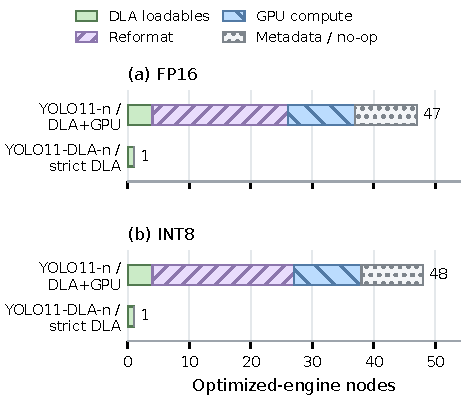
\includegraphics[width=\columnwidth]{figures/engine_composition.pdf}
\caption{Optimized-engine composition in FP16 and INT8. Counts are taken from
TensorRT engine-inspector outputs and represent DLA loadables, reformat nodes,
GPU compute nodes, and metadata/no-op nodes. In both precisions, YOLO11-n with
DLA+GPU execution remains partitioned across four DLA loadables with interleaved
GPU and reformat nodes, whereas strict YOLO11-DLA-n forms one DLA loadable with
no GPU or reformat nodes. These counts describe optimized-engine nodes, not
source-layer assignments or profiler records.}
\label{fig:composition}
\end{figure}

Figure~\ref{fig:composition} shows that the optimized-engine structure is nearly
unchanged by precision. YOLO11-n with DLA+GPU execution contains four DLA
loadables, eleven GPU compute nodes, and 22/23 reformat nodes in FP16/INT8,
whereas strict \model\ remains one DLA loadable with no GPU or reformat nodes
in both modes.
Comparing these heterogeneous deployments with strict DLA includes changed
attention and output boundaries and does not isolate partitioning cost.

\subsection{Engine-Plus-Transfer Latency}
\label{sec:engine}
The \texttt{trtexec} microbenchmark uses a 2\,s warm-up, a 30\,s timing window,
one inference stream, spin waiting, generated input data, and transfers enabled:
\begin{equation}
 L_{\mathrm{engine+IO}}=T_{\mathrm{H2D}}+T_{\mathrm{device}}+T_{\mathrm{D2H}}.
 \label{eq:latency}
\end{equation}
This boundary excludes preprocessing, host-side decoding, and NMS.
The reported percentiles describe frame variation within
each test, not confidence intervals across independent trials.

Table~\ref{tab:latency} shows that INT8 reduces strict DLA
median engine-plus-transfer latency from 27.515 to 4.167\,ms, a $6.60\times$ speedup. Strict DLA has lower
engine-plus-transfer latency than stock fallback in both modes: 20.7\% lower
median in FP16 and a $3.14\times$ reduction in INT8. The same adapted model on
GPU remains faster at this boundary: 3.500\,ms in FP16 and 2.828\,ms in INT8. Accuracy and application-pipeline costs are examined next.

\begin{figure*}[!t]
\centering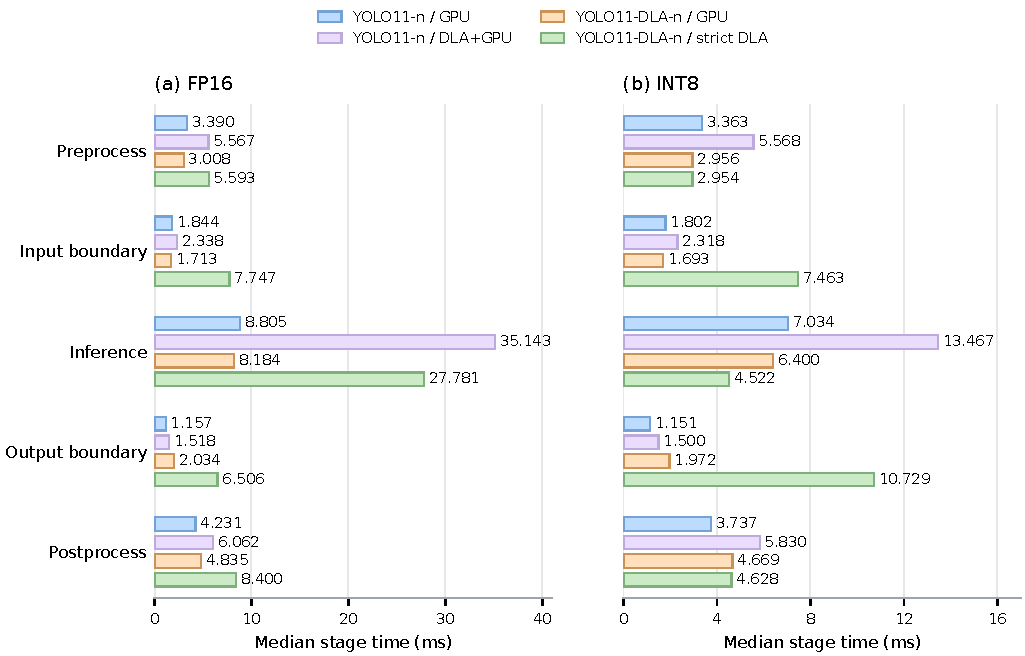
\includegraphics[width=\textwidth]{figures/application_stages.pdf}
\caption{Application-stage medians for all eight configurations under the same application workload. Panels use different horizontal scales. Input boundary
includes packing, quantization where needed, and H2D transfer; output boundary
includes D2H transfer, unpacking, and dequantization where needed. Inference
includes runtime launch and synchronization. Postprocess includes decoding and
NMS. Stage medians do not necessarily sum to the median total latency.}
\label{fig:stages}
\end{figure*}

\subsection{Deployed-Engine Accuracy}
\label{sec:accuracy}
The main comparison evaluates all eight configurations on the same 4,500
held-out images. Preprocessing centers a square $640\times640$ letterbox with padding
114 and RGB normalization by 255. CPU post-processing uses confidence 0.001,
class-aware NMS at intersection over union (IoU) 0.7, multi-label candidates,
and at most 300 boxes per image; COCOeval uses standard detection limits.
These settings differ from the timing thresholds.

\begin{table}[!b]
\caption{Accuracy on 4,500 held-out COCO val2017 images, disjoint from INT8 calibration. AP values are percentage points; INT8 allows mixed precision; stock and adapted training budgets differ.}
\label{tab:accuracy}\centering\footnotesize
\setlength{\tabcolsep}{3pt}
\begin{tabular*}{\columnwidth}{@{\extracolsep{\fill}}lllrrr@{}}
\toprule
Model & Device & Mode & AP & AP$_{50}$ & AP$_{75}$ \\
\midrule
YOLO11-n & GPU & FP16 & 39.378 & 55.190 & 42.845 \\
YOLO11-n & DLA+GPU & FP16 & 39.308 & 55.160 & 42.823 \\
YOLO11-DLA-n & GPU & FP16 & 37.879 & 53.633 & 41.008 \\
YOLO11-DLA-n & DLA & FP16 & 37.876 & 53.614 & 41.016 \\
\midrule
YOLO11-n & GPU & INT8 & 33.175 & 47.324 & 36.069 \\
YOLO11-n & DLA+GPU & INT8 & 19.827 & 35.241 & 20.867 \\
YOLO11-DLA-n & GPU & INT8 & 35.951 & 51.063 & 39.323 \\
YOLO11-DLA-n & DLA & INT8 & 35.408 & 50.790 & 38.614 \\
\bottomrule
\end{tabular*}
\end{table}
Table~\ref{tab:accuracy} compares precision and placement using the same images.
Strict INT8 loses 2.468 AP points relative to strict FP16; adapted GPU loses
1.928 points. Within a precision mode, strict DLA minus adapted GPU AP is
$-0.003$ points in FP16 and $-0.543$ in INT8. Thus, the negligible FP16
placement difference does not extend unchanged to INT8.
Stock GPU loses 6.203 points, while stock fallback loses 19.48 AP points,
reaching only 19.827 AP. Under this calibration protocol, the adapted INT8
engines exceed stock INT8 accuracy, but the fallback result is not an
accuracy-equivalent baseline. These tests do not isolate the cause of its
accuracy loss. Architecture, training, and calibration can all affect the
comparison, so this ordering cannot be assumed for other quantization setups.

\subsection{Multi-Image Application Pipeline}
\label{sec:application}
The sequential runtime cycles through a fixed subset of COCO val2017 for 60\,s after 30 warm-up frames and 30\,s stabilization. CPU preprocessing and NMS use one
thread, confidence 0.25, single-label candidates, and NMS IoU 0.45; adapted
engines use sparse decoding.
The boundary includes preprocessing, native I/O and any quantization/dequantization,
inference, decode, and NMS; it excludes disk access, visualization, and camera acquisition.

INT8 reduces strict DLA median application-pipeline latency from 56.820 to 30.675\,ms,
a $1.85\times$ speedup (Table~\ref{tab:latency}). The engine-level speedup is larger.
Figure~\ref{fig:stages} shows that the measured INT8 inference stage is faster
on strict DLA than on the adapted GPU engine (4.522 versus 6.400\,ms), but
strict DLA input and output boundaries take 7.463 and 10.729\,ms, respectively.
Each boundary exceeds the inference stage itself.
Native DLA layouts introduce an additional boundary cost in the evaluated host
implementation. The layout requirement is structural, while the magnitude of
packing and unpacking overhead is implementation-dependent. Because adapted
GPU and strict DLA use the same surrounding preprocessing, decoder, and NMS
implementation, their application-level comparison exposes this additional
boundary cost in the evaluated system.

The engine ordering reverses at the application boundary in both modes:
strict latency exceeds fallback by 10.9\% in FP16 and 5.7\% in INT8. Adapted
INT8 GPU is faster still, at 18.212\,ms.

\subsection{Module Energy at a Matched Delivered Rate}
\label{sec:energy}
Energy tests use the same application workload at 10\,Hz for 60\,s, with the
application thresholds and warm-up/stabilization protocol above. Every active
configuration completes 600 frames without observed drops or
misses of the 100\,ms release-to-result deadline.

\begin{figure*}[!t]
\centering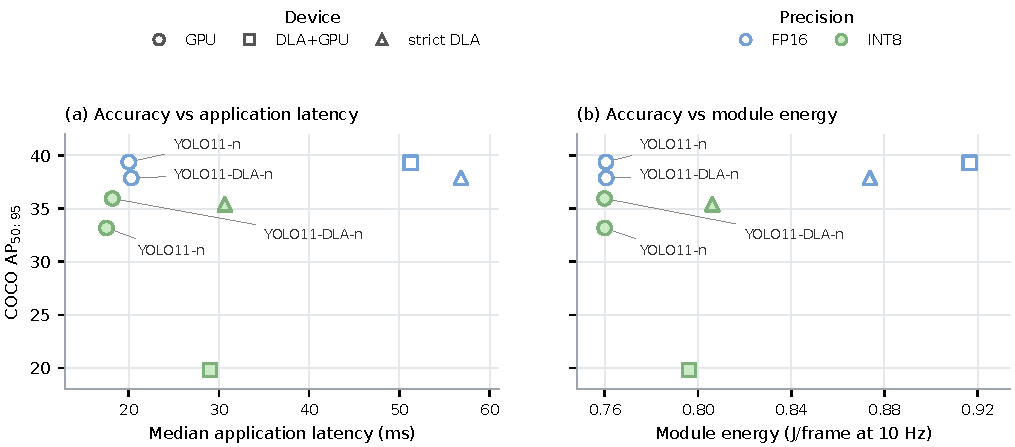
\includegraphics[width=\textwidth]{figures/deployment_tradeoffs.pdf}
\caption{Deployment trade-offs for all eight configurations: held-out COCO AP
versus application latency and module energy at 10\,Hz. Marker shapes identify
GPU, DLA+GPU, and strict DLA deployment; open and filled markers denote FP16
and INT8, respectively. Strict DLA provides verified learned-graph placement
without GPU-assigned learned layers, a property not represented by either
quantitative axis.}
\label{fig:tradeoffs}
\end{figure*}

Module power sums the non-overlapping \texttt{VDD\_GPU\_SOC},
\texttt{VDD\_CPU\_CV}, and \texttt{VIN\_SYS\_5V0} rails, excluding wall-plug
and whole-carrier consumption. Module energy per frame is
\begin{equation}
 E_{\mathrm{frame}}=\frac{\int_{t_0}^{t_1}P_{\mathrm{module}}(t)\,dt}
 {N_{\mathrm{completed}}}.
 \label{eq:energy}
\end{equation}
Separate idle measurements for each precision are subtracted over each active
interval to obtain incremental energy.
The measurement covers the whole module, including the CPU stages around the
accelerator, and is not a measurement of DLA core efficiency.

\begin{table}[t]
\caption{Module energy at 10\,Hz, 600 frames per test. Total and idle-subtracted energy: J/frame.}
\label{tab:energy}\centering\footnotesize
\setlength{\tabcolsep}{3pt}
\begin{tabular*}{\columnwidth}{@{\extracolsep{\fill}}lllrr@{}}
\toprule
Model & Device & Mode & \shortstack{Total\\J/frame} & \shortstack{Idle-subtracted\\J/frame} \\
\midrule
YOLO11-n & GPU & FP16 & 0.761 & 0.060 \\
YOLO11-n & DLA+GPU & FP16 & 0.917 & 0.216 \\
YOLO11-DLA-n & GPU & FP16 & 0.761 & 0.060 \\
YOLO11-DLA-n & DLA & FP16 & 0.874 & 0.174 \\
\midrule
YOLO11-n & GPU & INT8 & 0.760 & 0.060 \\
YOLO11-n & DLA+GPU & INT8 & 0.796 & 0.096 \\
YOLO11-DLA-n & GPU & INT8 & 0.760 & 0.060 \\
YOLO11-DLA-n & DLA & INT8 & 0.806 & 0.106 \\
\bottomrule
\end{tabular*}
\end{table}
Strict INT8 uses 0.806\,J/frame, 7.7\% below strict FP16, but 6.1\% above
adapted INT8 GPU (Table~\ref{tab:energy}). Whereas strict FP16 uses 4.7\% less
energy than stock FP16 fallback, strict INT8 is slightly higher than its
fallback counterpart (0.796\,J/frame), whose accuracy is much lower.
GPU module energy remains approximately 0.760--0.761\,J/frame in both modes.
These results apply to the measured 10\,Hz operating point. Small differences
and idle-subtracted values remain sensitive to baseline stability.

Figure~\ref{fig:tradeoffs} summarizes the deployment trade-offs. For each DLA
configuration, a GPU configuration offers higher AP with lower application
latency and lower module energy. Strict DLA instead provides verified placement
without GPU-assigned learned layers, a property outside these quantitative axes.

